% Chapter Template

\chapter{Ensayos y Resultados} % Main chapter title

\label{Chapter4} % Change X to a consecutive number; for referencing this chapter elsewhere, use \ref{ChapterX}

%----------------------------------------------------------------------------------------
%	SECTION 1
%----------------------------------------------------------------------------------------

En esta sección se presentan los ensayos realizados, los resultados obtenidos y el análisis correspondiente.

\section{Dispositivos desarrollados}
En la figura \ref{fig:MainBoaard} se puede observar el resultado del diseño de la tarjeta. Esta se encuentra armada con los módulos insertables Sigfox y LoRa y fue sometida a diferentes ensayos indicados en la sección \ref{sec:pruebasHW} 

\begin{figure}[H]
	\centering
	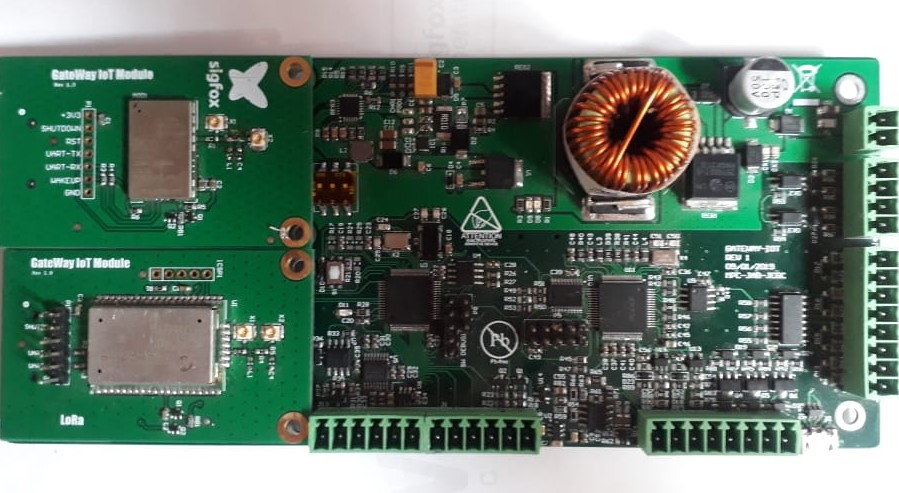
\includegraphics[scale=.45]{./Figures/MainBoardCompleta.jpeg}
	\caption{Tarjeta principal armada con los módulos Sifox y LoRa.}
	\label{fig:MainBoaard}
\end{figure}


\section{Pruebas de hardware sobre el prototipo} \label{sec:pruebasHW}
A la tarjeta se le hicieron pruebas individuales de hardware:
\begin{itemize}
    \item Cortos y continuidades.
    \item Voltaje en la linea de alimentación.
    \item Test visual comparado con el plano de ensamble, (ver figura
    \ref{fig:Planoensamble}.)
\end{itemize}

\begin{figure}[H]
	\centering
	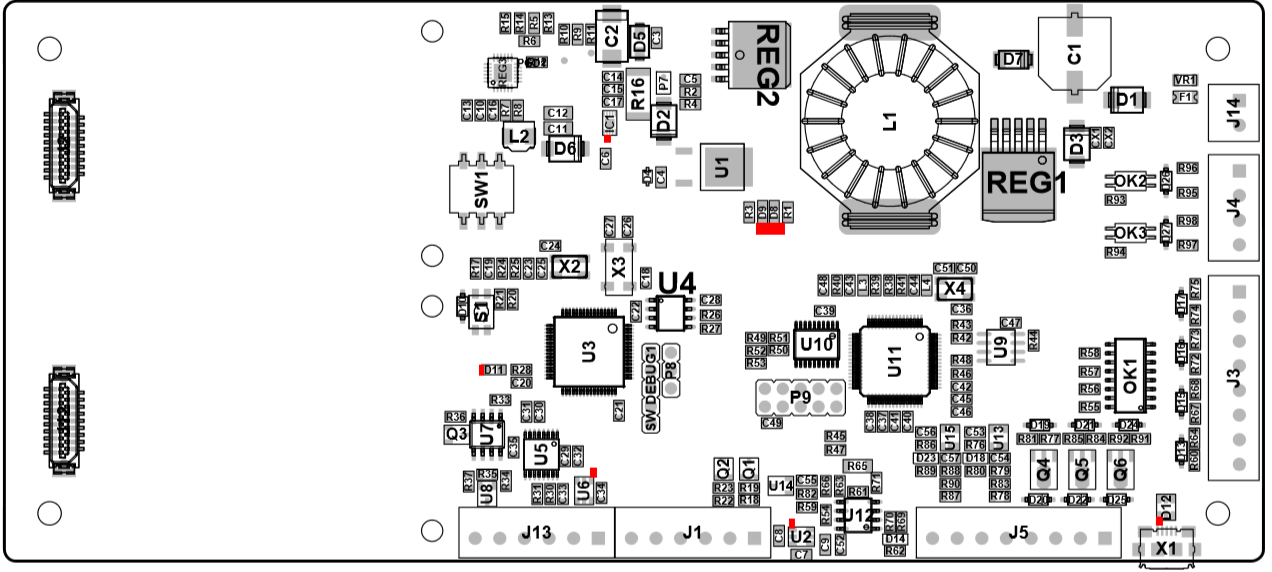
\includegraphics[scale=.45]{./Figures/Planoensamble.PNG}
	\caption{Plano de ensamble tarjeta principal.}
	\label{fig:Planoensamble}
\end{figure}

\section{Resultados de sintonización y verificación de la antena Sigfox}
En la ecuación \ref{eq:Impedancia2} y \ref{eq:Impedancia3} se pueden observar los valores de la impedancia y RL medidos con el VNA para una frecuencia de 915.516625 MHz.

En la figura \ref{fig:tunnigsigfoxchart} se puede observar el resultado de la verificación de la antena con el VNA, donde el marcador se encuentra muy cerca al origen de la carta de Smith y al eje real. Lo ideal en la sintonización es que el valor de la resistencia se acerque a \SI{50}{\ohm} y el valor de la reactancia (parte imaginaria \textit{j} de la ecuación \ref{eq:Impedancia2}) sea lo mas cercano a \SI{0}{\ohm} para garantizar la mejor eficiencia y la menor reflexión posible.

En la figura \ref{fig:tunnigsigfox5} se puede observar los resultados de la curva de perdidas de retorno. Esta deja evidenciar que tiene un ancho de banda de aproximadamente 125 KHz, el cual se mide a partir de -10dB\citep{AntenaSigFox2016}.


\begin{equation}
	\label{eq:Impedancia2}
	Z = 37.5\SI{}{\ohm} - j*4.7\SI{}{\ohm}
\end{equation}
\begin{equation}
	\label{eq:Impedancia3}
    RL = -16.35 dB
\end{equation}

\begin{figure}[H]
	\centering
	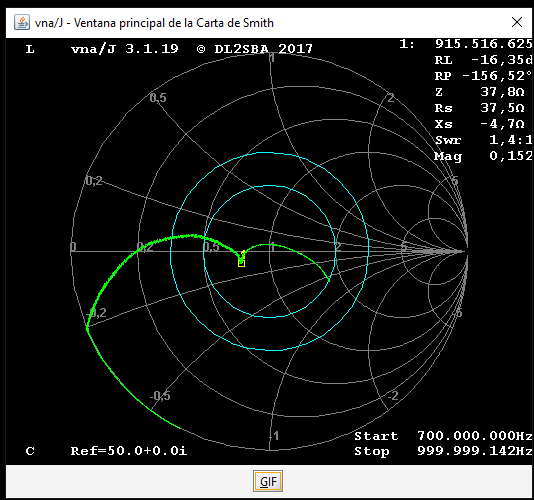
\includegraphics[scale=.7]{./Figures/tunnigsigfoxchart.png}
	\caption{Carta de Smith 915 MHz.}
	\label{fig:tunnigsigfoxchart}
\end{figure}

\begin{figure}[H]
	\centering
	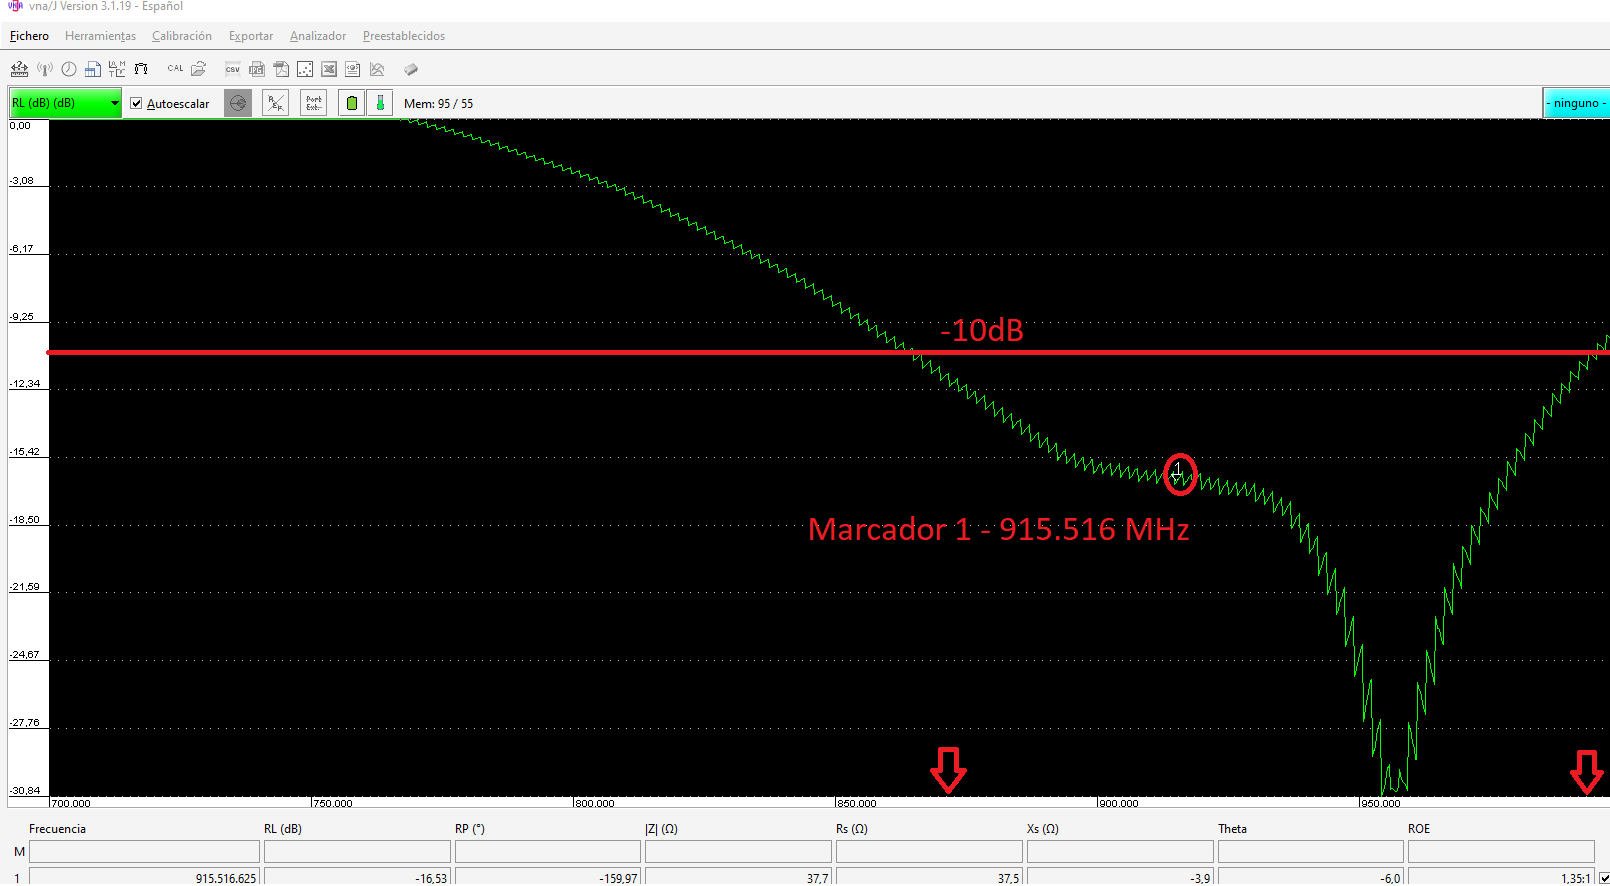
\includegraphics[scale=.35]{./Figures/tunnigsigfox5.png}
	\caption{Perdidas de retorno a 915 MHz.}
	\label{fig:tunnigsigfox5}
\end{figure}


%  Este valor de impedancia se encuentra muy cercano al eje real (37.5\SI{}{\ohm}). Entre mas cercano al eje real  y el valor de la reactancia X sea lo mas cercano a 0\SI{}{\ohm} habrán menos perdidos por reflexión. 


\section{Resultados de pruebas funcionales sobre  los módulos}

Los módulos Sigfox y LoRa se probaron individualmente, enviándole comandos AT y comandos MAC respectivamente. Con esto se verificó la correcta funcionalidad del dispositivo.
%y la verificación de consumos de corriente en modo \textit{Sleep}. 

% \begin{figure}[H]
% 	\centering
% %	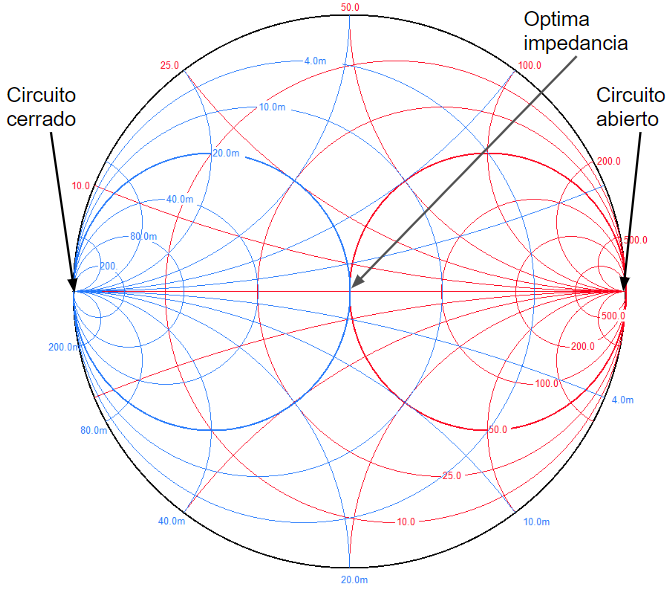
\includegraphics[scale=.45]{./Figures/CartaSmith.png}
% 	\caption{Consumo de corriente modulo Wisol - Sigfox.}
% 	\label{fig:ConsumoWisol}
% \end{figure}

% \begin{figure}[H]
% 	\centering
% %	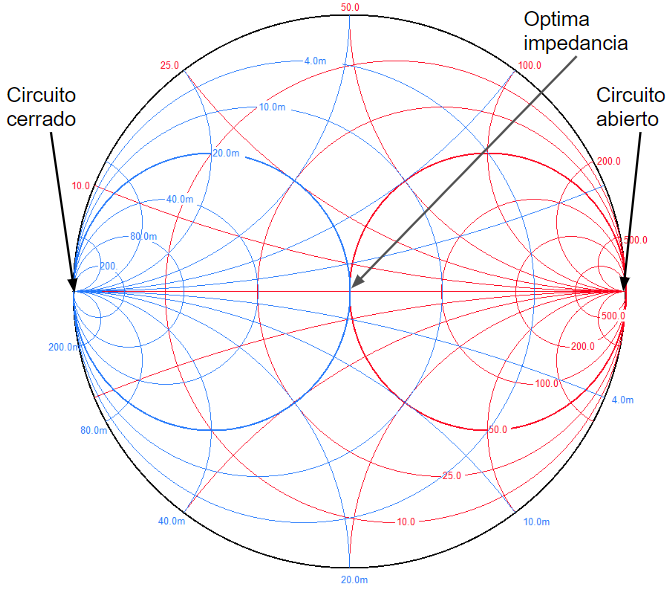
\includegraphics[scale=.45]{./Figures/CartaSmith.png}
% 	\caption{Consumo de corriente modulo RN2903 - LoRaWAN.}
% 	\label{fig:ConsumoLoraWAN}
% \end{figure}
\subsubsection{Resultados de las pruebas de transmisión de Sigfox}
Para la verificación de las transmisiones se uso el \textit{Back-end} Sigfox para la visualización de los paquetes de datos enviados.

En la figura \ref{fig:COMANDOSATSIGFOX} se pueden observar los comandos enviados al modulo Sigfox. En la figura \ref{fig:tRANSMISIONsIGFOX} se puede observar el mensaje de prueba visto en la plataforma de Sigfox. También se visualiza la cantidad (15) de estaciones bases que vieron el dispositivo y la cantidad de reenvíos (\textit{frames}), en 9 de 15 antenas se recibieron 3 de 3 paquetes enviados, por defecto Sigfox  envía tres \textit{frames} en cada transmisión y cada antena los recibe dependiendo de lo alejado que se encuentre el dispositivo de la estación base.

\begin{figure}[H]
	\centering
	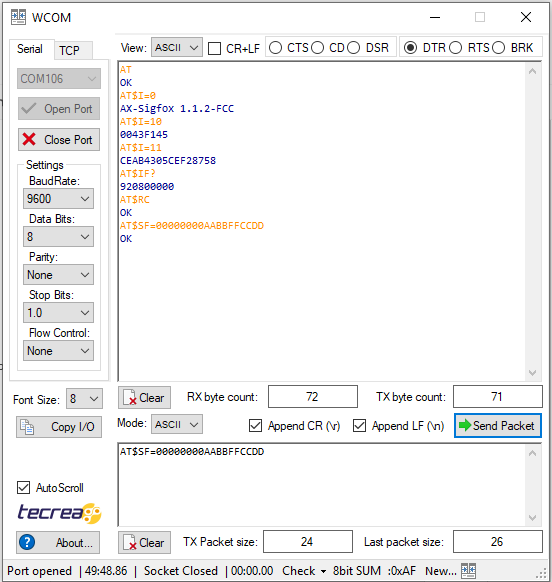
\includegraphics[scale=.5]{./Figures/COMANDOSATSIGFOX.PNG}
	\caption{Comandos enviados al módulo Wisol-Sigfox.}
	\label{fig:COMANDOSATSIGFOX}
\end{figure}
\begin{figure}[H]
	\centering
	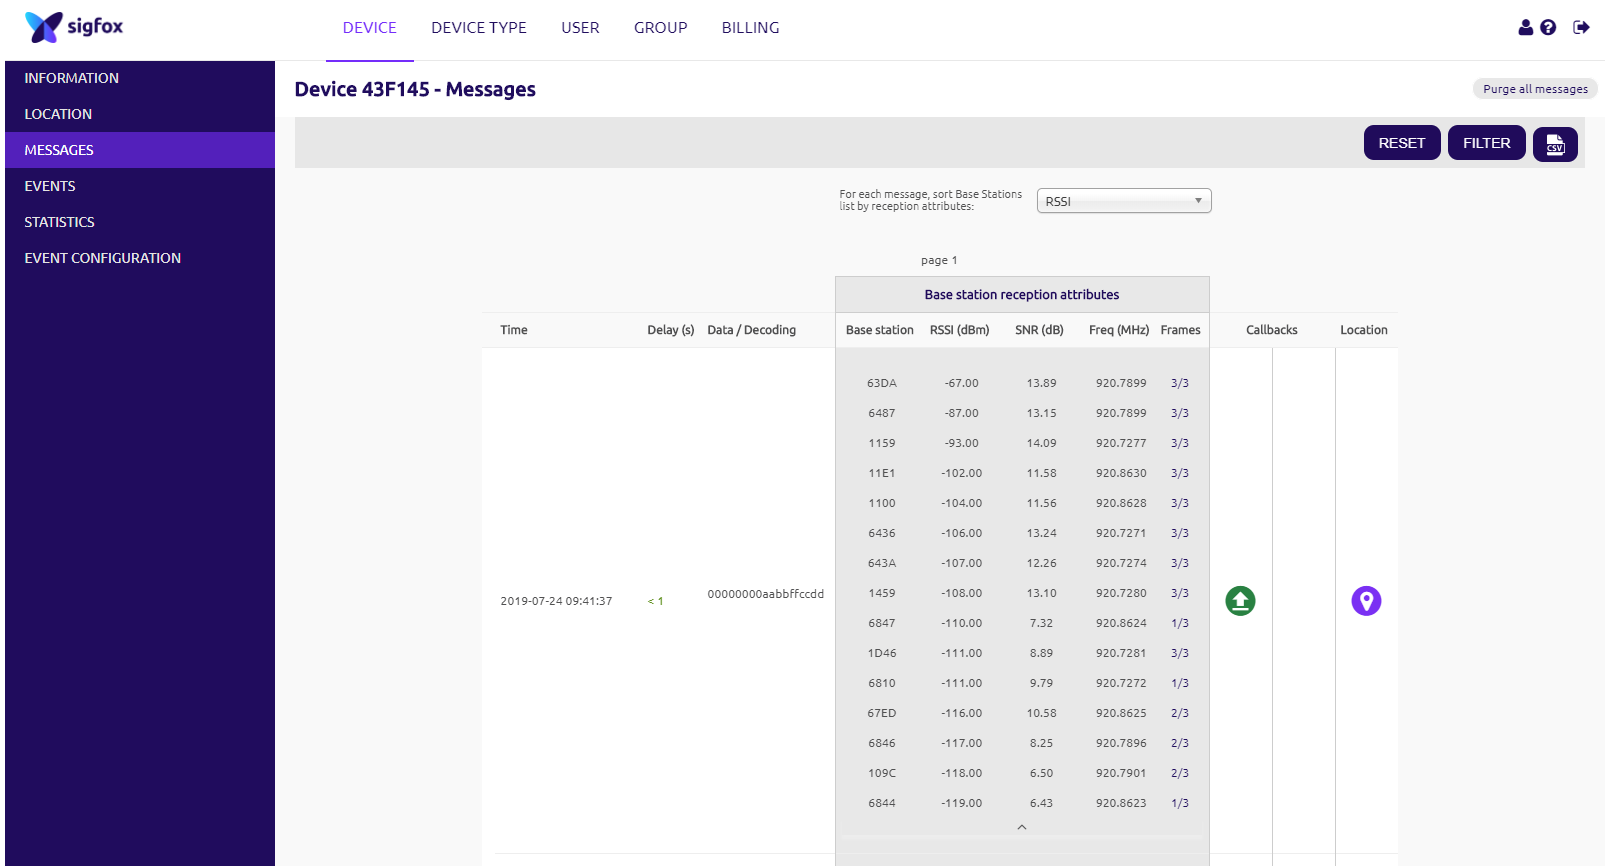
\includegraphics[scale=.35]{./Figures/tRANSMISIONsIGFOX.PNG}
	\caption{Prueba de transmisiones de mensajes de subida Sigfox.}
	\label{fig:tRANSMISIONsIGFOX}
\end{figure}

El dispositivo se alejo 10 Km del lugar de donde inicialmente se realizaron las transmisiones. En la figura \ref{fig:AntenasSigfoxAlejada} se puede observar que la cantidad (8 a 10) de estaciones base que vieron el dispositivo.
\begin{figure}[H]
	\centering
	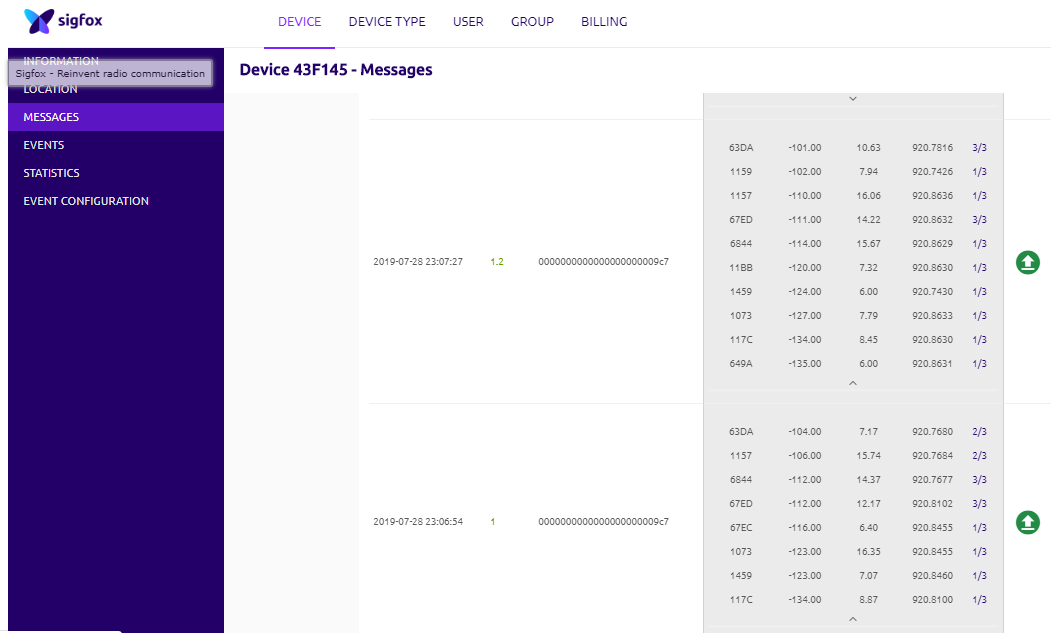
\includegraphics[scale=.45]{./Figures/AntenasSigfoxAlejada.PNG}
	\caption{Transmisiones de mensajes Sigfox a 10Km de distancia.}
	\label{fig:AntenasSigfoxAlejada}
\end{figure}

\subsubsection{Resultados de las pruebas de transmisión de LoRaWAN}

En la figura \ref{fig:ComandMacLora} se pueden observar los comandos enviados al modulo LoRaWAN. Para la verificación de las transmisiones de loRaWAN se usó el servidor \textit{the things network} para la visualización de los paquetes de datos enviados (ver figura \ref{fig:Datalorawantest}).


\begin{figure}[H]
	\centering
	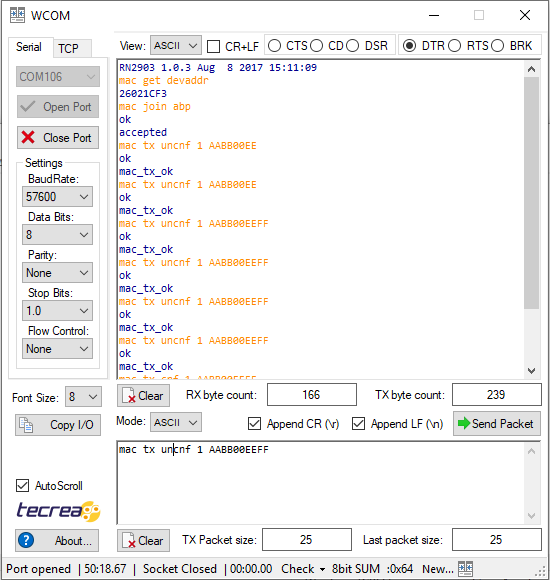
\includegraphics[scale=.45]{./Figures/ComandMacLora.PNG}
	\caption{Comandos enviados al módulo LoRaWAN.}
	\label{fig:ComandMacLora}
\end{figure}
\begin{figure}[H]
	\centering
	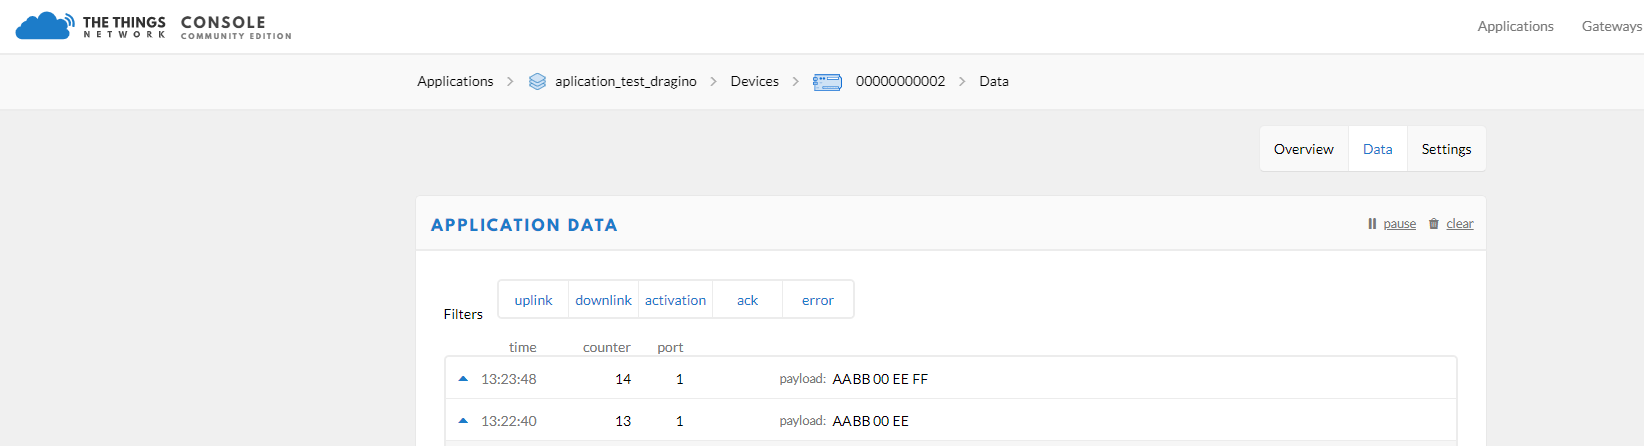
\includegraphics[scale=.35]{./Figures/Datalorawantest.PNG}
	\caption{Prueba de transmision de mensajes con LoRaWAN.}
	\label{fig:Datalorawantest}
\end{figure}

En la figura \ref{fig:LoraTX_corto} se puede observar que de 156 mensajes transmitidos con el dispositivo a una distancia menor a 1m del gateway. Solo 6 mensajes fueron recibidos por el servidor.
\begin{figure}[H]
	\centering
	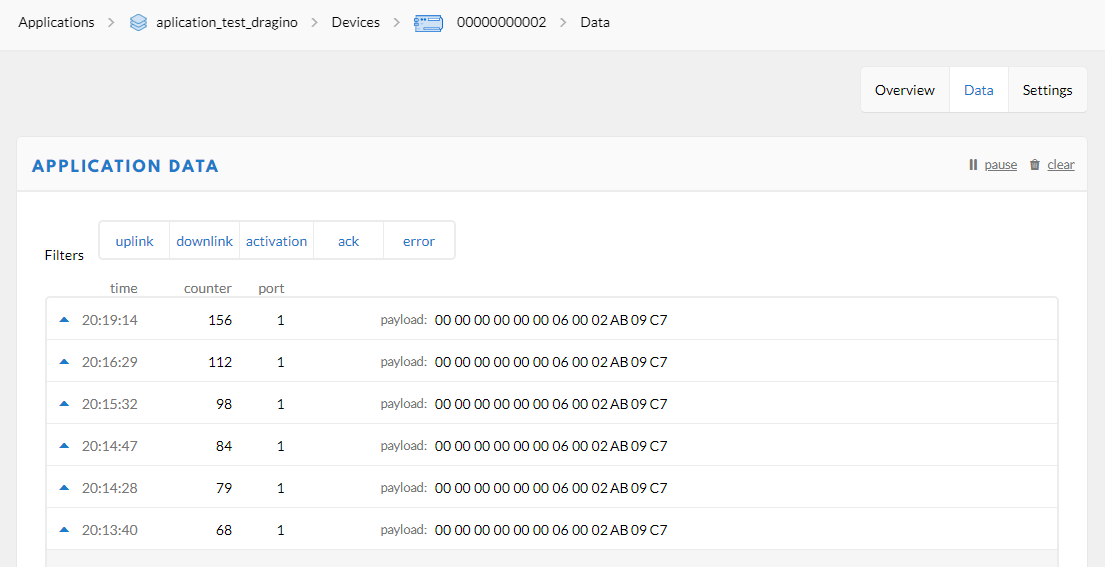
\includegraphics[scale=.5]{./Figures/LoraTX_corto.PNG}
	\caption{Cuantificación de mensajes enviados con LoRaWAN.}
	\label{fig:LoraTX_corto}
\end{figure}
%\footnotetext{\url{https://www.thethingsnetwork.org/}}

\section{Pruebas de consumo de energía}
Los módulos LoRaWAN y Sigfox trabajan bajo redes LPWAN, por lo que el consumo debe ser lo más bajo posible. Esto debido a que en las aplicaciones se busca que los dispositivos finales tengan una durabilidad de muchos años. En la tabla \ref{tab:ConsumosTabla} se pueden observar los datos de los consumos usados.

\begin{table}[h]
	\centering
	\caption[Consumos]{Medición de consumos energéticos Sigfox y LoRaWAN }
	\begin{tabular}{l c c}    
		\toprule
		\textbf{ \textit{Modo} } & \textbf{Sigfox} & \textbf{LoRaWAN} \\
		\midrule
		Normal	    &$\mathrm{0.53 mA}$ 	&$\mathrm{6.71 mA}$  \\	
		\textit{Sleep}	            & $\mathrm{0.3 \mu{A}}$     & $\mathrm{6.4 \mu{A}}$\\
		\bottomrule
		\hline
	\end{tabular}
	\label{tab:ConsumosTabla}
\end{table}


El consumo energético del modulo Sigfox WWSFM11R2D se puede observar en la figura \ref{fig:Consumo_SigNormal} y \ref{fig:ConsumoSigSleep}. 
\begin{figure}[H]
	\centering
	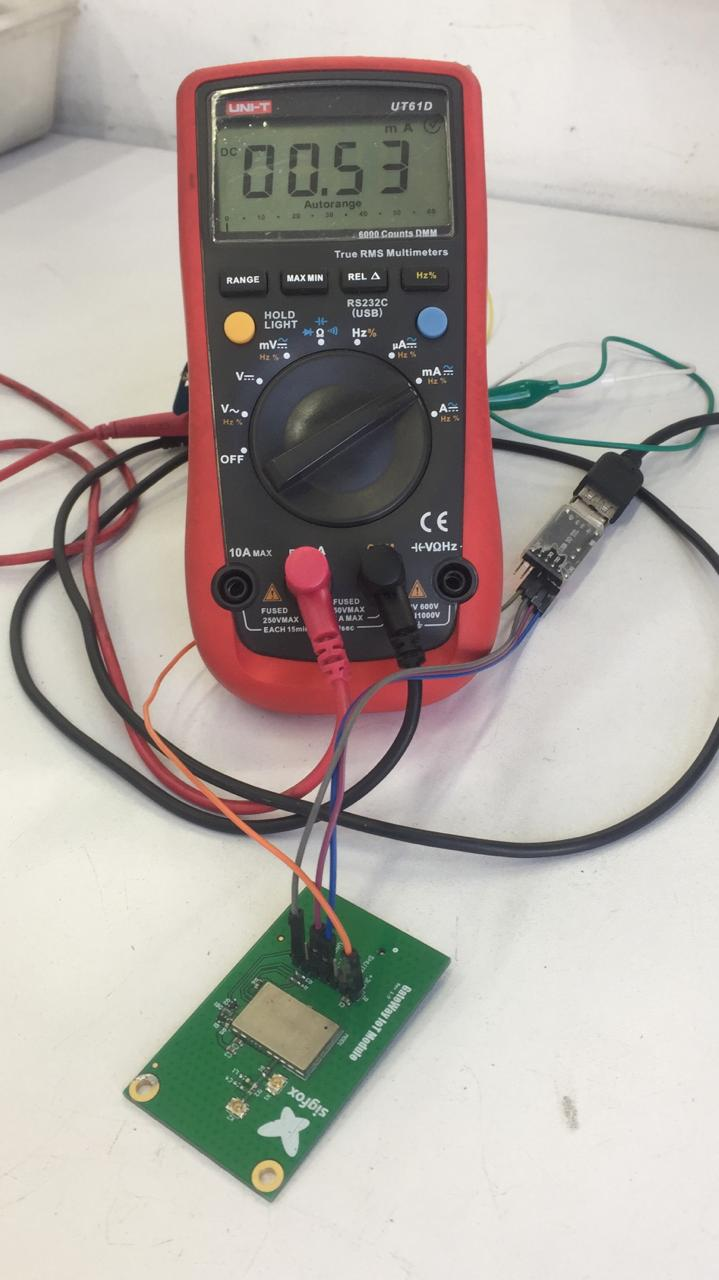
\includegraphics[scale=.15]{./Figures/Consumo_SigNormal.jpeg}
	\caption{Consumo de WWSFM11R2D en funcionamiento normal.}
	\label{fig:Consumo_SigNormal}
\end{figure}

\begin{figure}[H]
	\centering
	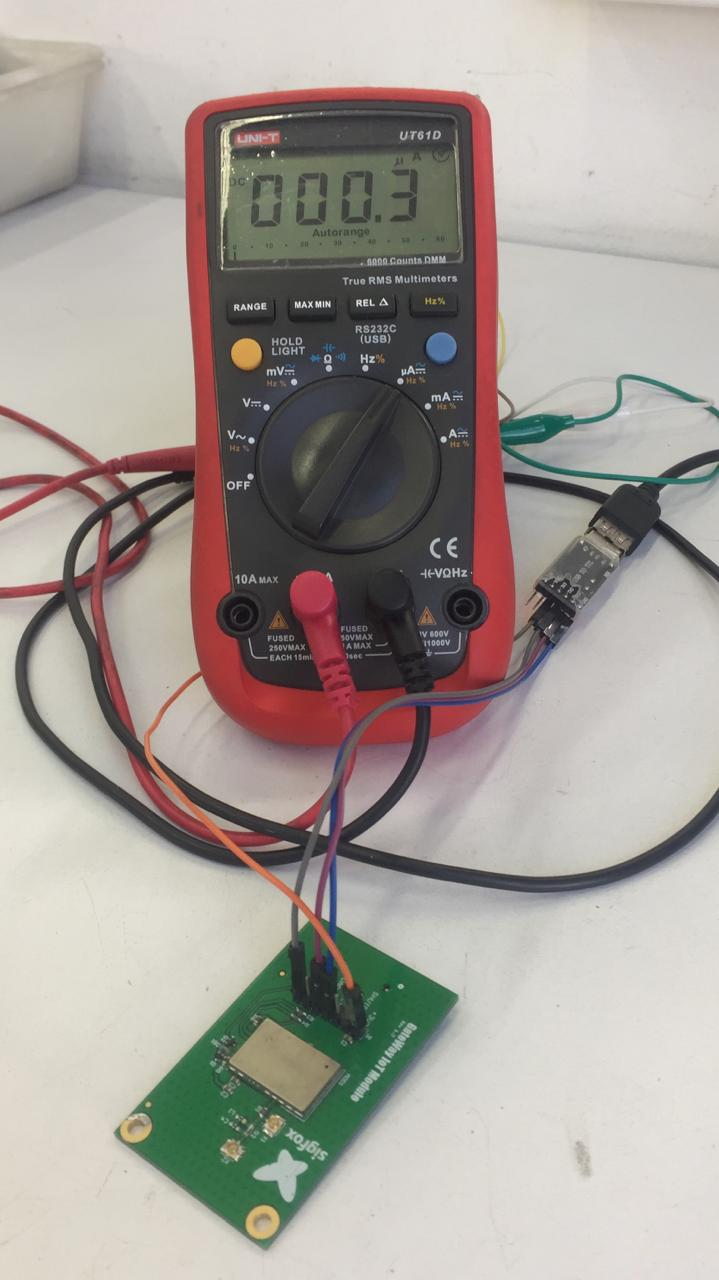
\includegraphics[scale=.15]{./Figures/ConsumoSigSleep.jpeg}
	\caption{Consumo de WWSFM11R2D en modo \textit{sleep}}
	\label{fig:ConsumoSigSleep}
\end{figure}

El consumo energético del modulo LoRaWAN se puede observar en la figura \ref{fig:ConsumoLoraNormal} y \ref{fig:ConsumoLoraSleep}. 

\begin{figure}[H]
	\centering
	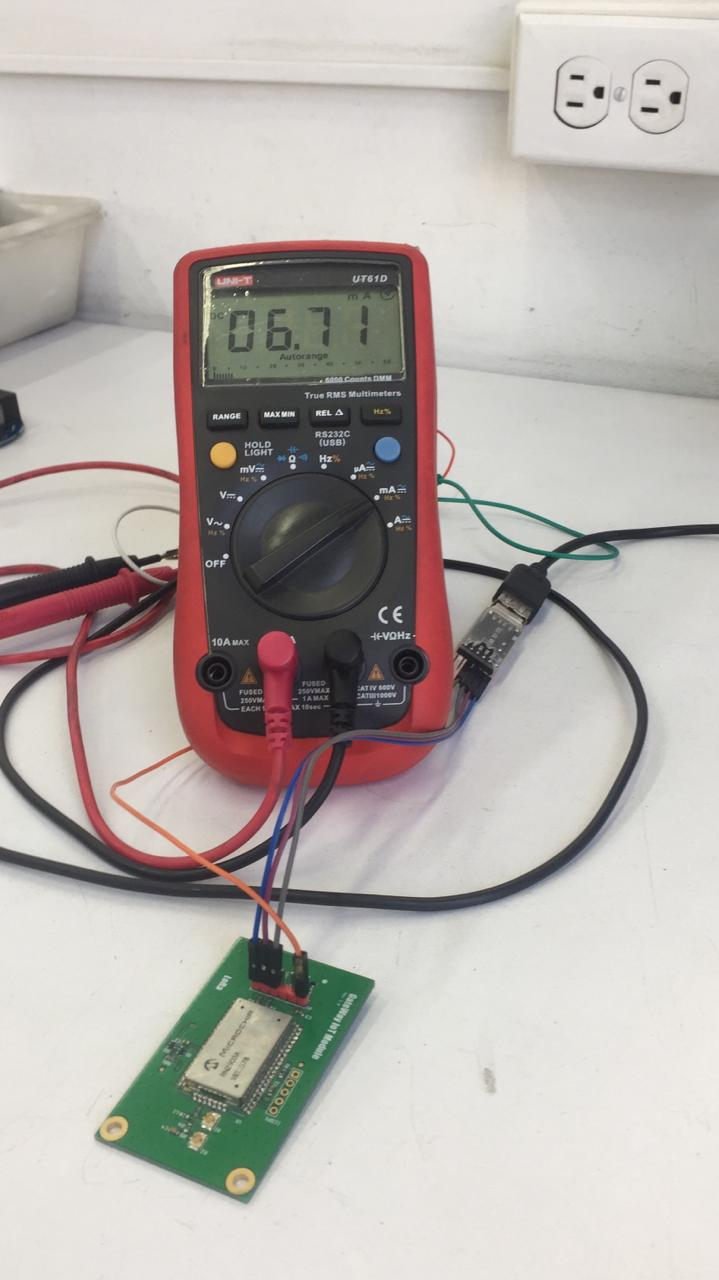
\includegraphics[scale=.15]{./Figures/ConsumoLoraNormal.jpeg}
	\caption{Consumo de RN2903 en funcionamiento normal.}
	\label{fig:ConsumoLoraNormal}
\end{figure}

\begin{figure}[H]
	\centering
	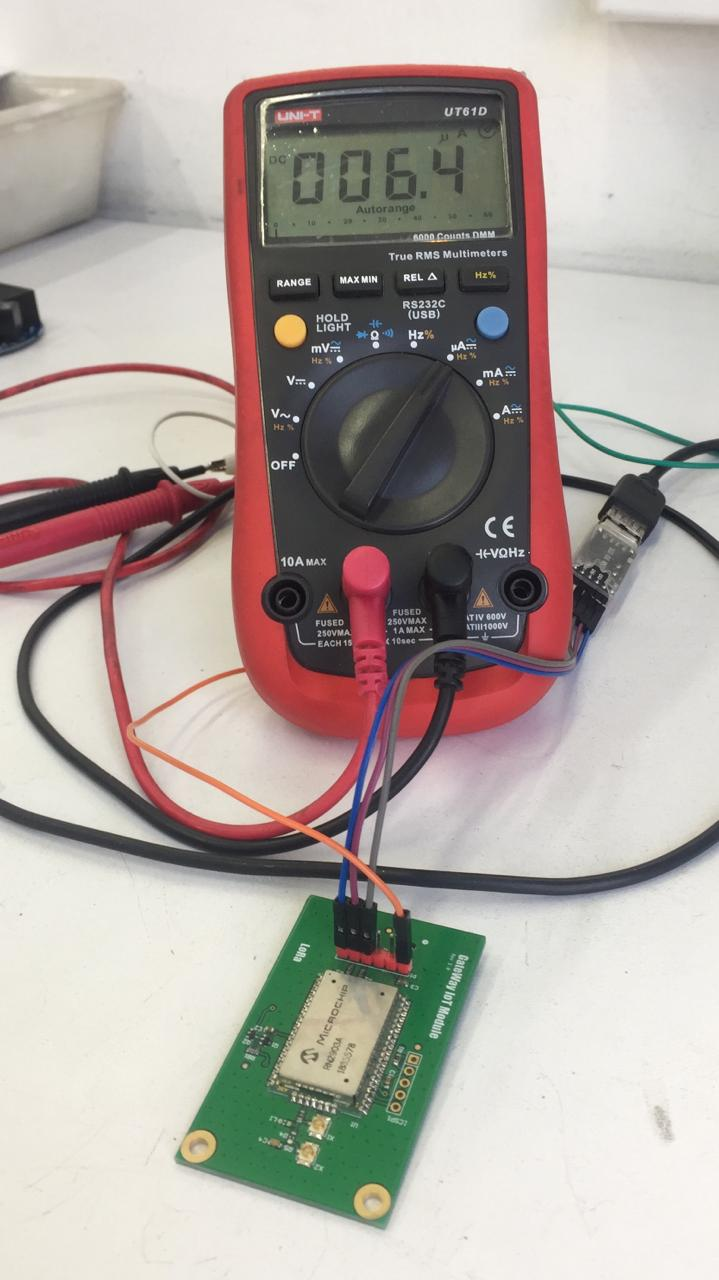
\includegraphics[scale=.15]{./Figures/ConsumoLoraSleep.jpeg}
	\caption{Consumo de RN2903 en modo \textit{sleep}}
	\label{fig:ConsumoLoraSleep}
\end{figure}

La medición de corriente en los módulos deja evidenciar que mientras se encuentra en modo de funcionamiento el consumo es alto, sin embargo cuando se les envía el comando para entrar en modo de bajo consumo la corriente baja considerablemente al orden de $\mu{A}$.


\section{Pruebas de integración}
Para las pruebas de integración se contó con :
\begin{itemize}
    \item Acceso remoto al servidor de Sigfox y LoRaWAN. 
    \item Acceso remoto a  la plataforma xxxx para no visualizar las señales en crudo.
    \item Acceso físico a los dispositivos embebidos
    \item Terminal serial WCOM desarrollada por Tecrea SAS.
    \item Multimetro UNI-T ut61D con resolución de hasta 100 nA.
    \item Acceso a consola serial de la tarjeta principal.
\end{itemize}

En la figura \ref{fig:IntegracionSL2} se puede observar la consola de depuracíon del dispositivo. Durante el proceso de pruebas permitió la visualización del estado interno de la aplicación embebida al mostrar los mensajes impresos por el firmware desarrollado. Se puede visualizar que el mensaje enviado es:

00 00 00 00 00 00 06 00 02 AB 09 c7 

Este se puede decodificar de acuerdo a la siguiente imagen \ref{fig:FRAME}, como cada canal analógico es de 12 bits, al valor de los canales ADC0, ADC1, ADC2 se les debe aplicar la formula \ref{eq:ADC} para obtener el resultado de 2.786 V, 4.5 V y 0 mA.

\begin{equation}
	\label{eq:ADC}
	VADCx = (ADCx -2340 ) / 58.5
\end{equation}

\begin{figure}[H]
	\centering
	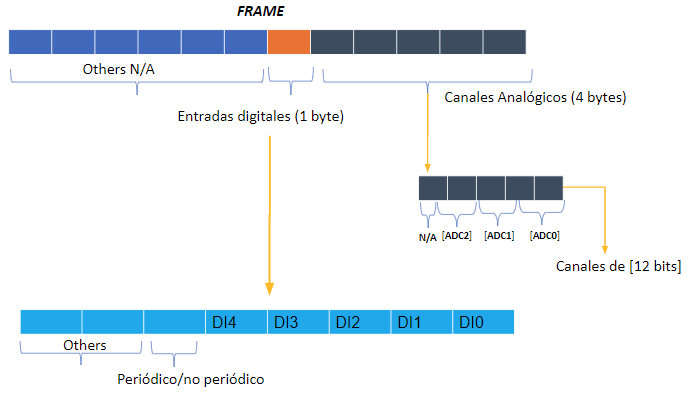
\includegraphics[scale=.6]{./Figures/FRAME.PNG}
	\caption{Codificación del paquete de datos.}
	\label{fig:FRAME}
\end{figure}

\begin{figure}[H]
	\centering
	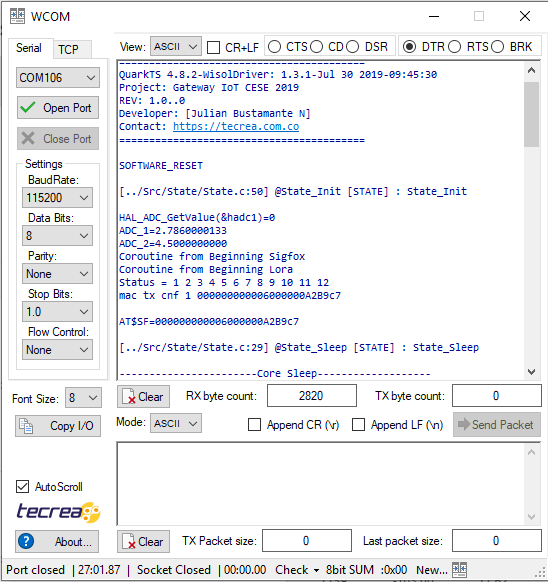
\includegraphics[scale=.6]{./Figures/IntegracionSL2.PNG}
	\caption{Consola de depuración del sistema embebido.}
	\label{fig:IntegracionSL2}
\end{figure}


En la figura \ref{fig:Ubidotsintegration} se puede observar la visualización del \textit{dashboard} con la medición de las variables en la plataforma Ubidots.

\begin{figure}[H]
	\centering
	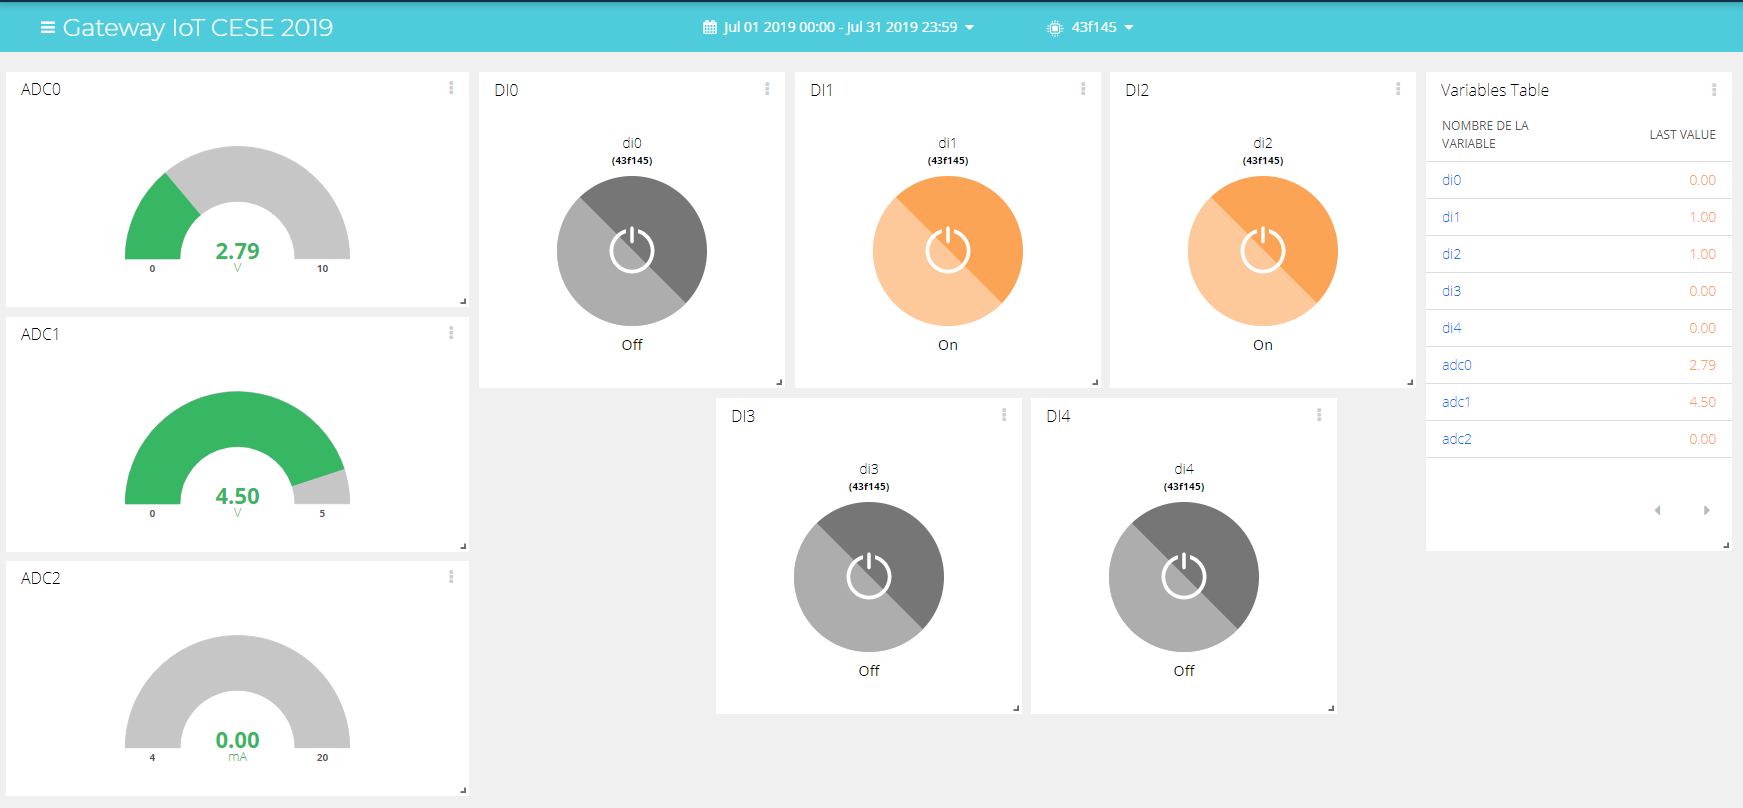
\includegraphics[scale=.3]{./Figures/Ubidotsintegration.PNG}
	\caption{Plataforma de integración.}
	\label{fig:Ubidotsintegration}
\end{figure}

%\section{Pruebas unitarias de manejadores de dispositivos (\textit{driver})}








